\subsection{Measurement Library Design}
\label{ss:dataflow}

NetMap uses a dedicated server for collecting and storing the performance
measurements (see figure \ref{fig:servers}), so game developers do not need to
worry about securely storing and forwarding the sensitive data, and do not need
to provision for the bandwidth required by the data uploads.

\begin{figure}[hbtp]
  \center{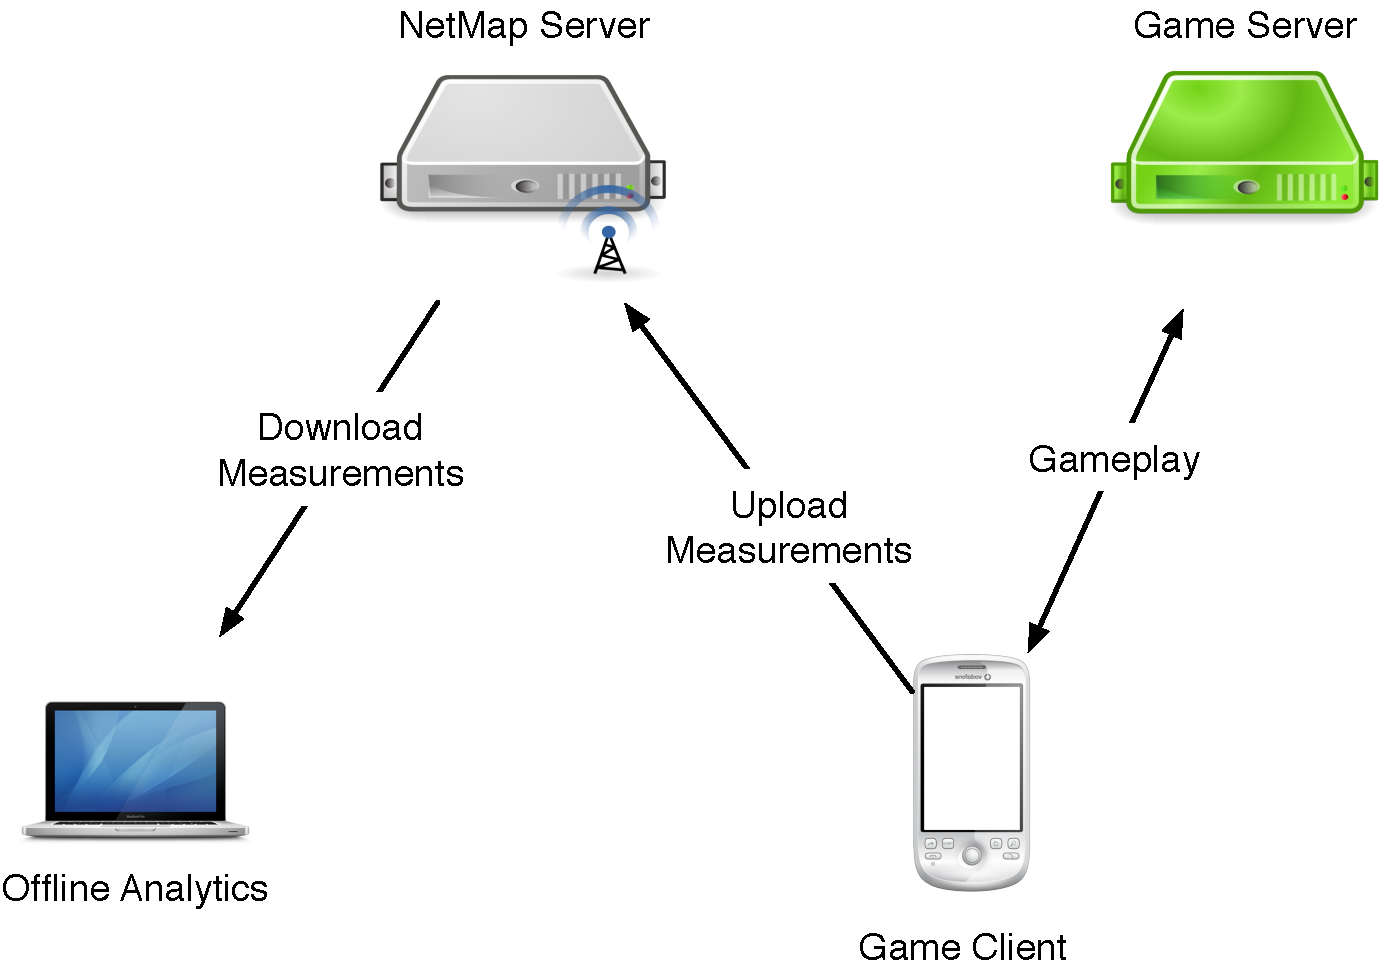
\includegraphics[width=85mm]{figures/servers.pdf}}
  \caption{
    The NetMap platform has a dedicated server for storing network
    performance measurements, and the data is analyzed offline.
  }
  \label{fig:servers}
\end{figure}

The NetMap platform includes an Android library that manages the
straight-forward (but tedious) aspects of measuring network performance and
uploading the data to the NetMap server. We envision that when a player takes
an action in a game, the game code will call our library and ask it to collect
a performance measurement. The measurement data is not uploaded to the NetMap
right away, so that the game can use all the player's (potentially limited)
wireless Internet bandwidth, so that the data upload is not charged against
the player's cellular Internet data quotas, and so that we do not burden the
player's mobile device battery. Instead, we queue up the data in a SQLite
database on the player's device, and we wait until the device is connected to a
WiFi network and its charger is plugged in. Under the right circumstances, all
the data queued up in SQLite is uploaded to the measurement server.

\begin{figure}[hbtp]
  \center{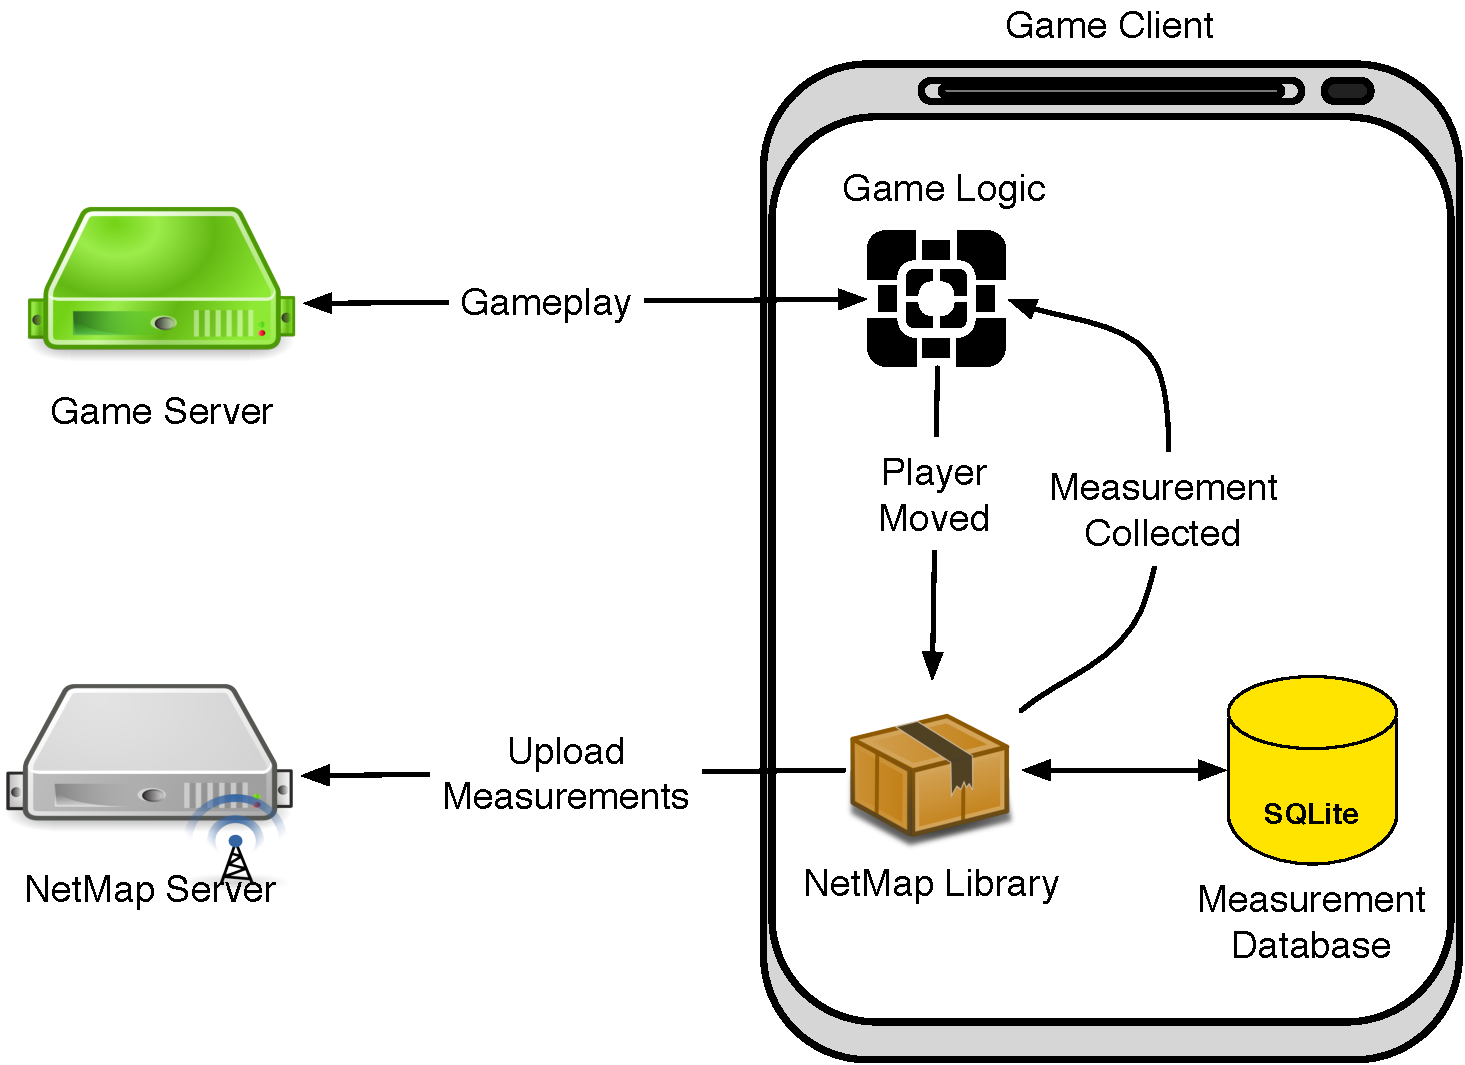
\includegraphics[width=85mm]{figures/dataflow.pdf}}
  \caption{
    The flow of measurement data inside a game client
  }
  \label{fig:dataflow}
\end{figure}




Powerful moves (such as firing a very powerful
weapon) would trigger the collection of more battery-intensive measurements.

